\ifx\allfiles\undefined
\documentclass[12pt, a4paper,oneside, UTF8]{ctexbook}
\usepackage[dvipsnames]{xcolor}
\usepackage{mathtools}   % 数学公式
\usepackage{amsthm}    % 定理环境
\usepackage{amssymb}   % 更多公式符号
\usepackage{graphicx}  % 插图
%\usepackage{mathrsfs}  % 数学字体
%\usepackage{newtxtext,newtxmath}
%\usepackage{arev}
\usepackage{kmath,kerkis}
\usepackage{newtxtext}
\usepackage{bbm}
\usepackage{enumitem}  % 列表
\usepackage{geometry}  % 页面调整
%\usepackage{unicode-math}
\usepackage[colorlinks,linkcolor=black]{hyperref}

\usepackage{wrapfig}


\usepackage{ulem}	   % 用于更多的下划线格式,
					   % \uline{}下划线,\uuline{}双下划线,\uwave{}下划波浪线,\sout{}中间删除线,\xout{}斜删除线
					   % \dashuline{}下划虚线,\dotuline{}文字底部加点


\graphicspath{ {flg/},{../flg/}, {config/}, {../config/} }  % 配置图形文件检索目录
\linespread{1.5} % 行高

% 页码设置
\geometry{top=25.4mm,bottom=25.4mm,left=20mm,right=20mm,headheight=2.17cm,headsep=4mm,footskip=12mm}

% 设置列表环境的上下间距
\setenumerate[1]{itemsep=5pt,partopsep=0pt,parsep=\parskip,topsep=5pt}
\setitemize[1]{itemsep=5pt,partopsep=0pt,parsep=\parskip,topsep=5pt}
\setdescription{itemsep=5pt,partopsep=0pt,parsep=\parskip,topsep=5pt}

% 定理环境
% ########## 定理环境 start ####################################
\theoremstyle{definition}
\newtheorem{defn}{\indent 定义}[section]

\newtheorem{lemma}{\indent 引理}[section]    % 引理 定理 推论 准则 共用一个编号计数
\newtheorem{thm}[lemma]{\indent 定理}
\newtheorem{corollary}[lemma]{\indent 推论}
\newtheorem{criterion}[lemma]{\indent 准则}

\newtheorem{proposition}{\indent 命题}[section]
\newtheorem{example}{\indent \color{SeaGreen}{例}}[section] % 绿色文字的 例 ,不需要就去除\color{SeaGreen}{}
\newtheorem*{rmk}{\indent \color{red}{注}}

% 两种方式定义中文的 证明 和 解 的环境:
% 缺点:\qedhere 命令将会失效【技术有限,暂时无法解决】
\renewenvironment{proof}{\par\textbf{证明.}\;}{\qed\par}
\newenvironment{solution}{\par{\textbf{解.}}\;}{\qed\par}

% 缺点:\bf 是过时命令,可以用 textb f等替代,但编译会有关于字体的警告,不过不影响使用【技术有限,暂时无法解决】
%\renewcommand{\proofname}{\indent\bf 证明}
%\newenvironment{solution}{\begin{proof}[\indent\bf 解]}{\end{proof}}
% ######### 定理环境 end  #####################################

% ↓↓↓↓↓↓↓↓↓↓↓↓↓↓↓↓↓ 以下是自定义的命令  ↓↓↓↓↓↓↓↓↓↓↓↓↓↓↓↓

% 用于调整表格的高度  使用 \hline\xrowht{25pt}
\newcommand{\xrowht}[2][0]{\addstackgap[.5\dimexpr#2\relax]{\vphantom{#1}}}

% 表格环境内长内容换行
\newcommand{\tabincell}[2]{\begin{tabular}{@{}#1@{}}#2\end{tabular}}

% 使用\linespread{1.5} 之后 cases 环境的行高也会改变,重新定义一个 ca 环境可以自动控制 cases 环境行高
\newenvironment{ca}[1][1]{\linespread{#1} \selectfont \begin{cases}}{\end{cases}}
% 和上面一样
\newenvironment{vx}[1][1]{\linespread{#1} \selectfont \begin{vmatrix}}{\end{vmatrix}}

\def\d{\textup{d}} % 直立体 d 用于微分符号 dx
\def\R{\mathbb{R}} % 实数域
\def\N{\mathbb{N}} % 自然数域
\def\C{\mathbb{C}} % 复数域
\def\Z{\mathbb{Z}} % 整数环
\def\Q{\mathbb{Q}} % 有理数域
\newcommand{\bs}[1]{\boldsymbol{#1}}    % 加粗,常用于向量
\newcommand{\ora}[1]{\overrightarrow{#1}} % 向量

% 数学 平行 符号
\newcommand{\pll}{\kern 0.56em/\kern -0.8em /\kern 0.56em}

% 用于空行\myspace{1} 表示空一行 填 2 表示空两行  
\newcommand{\myspace}[1]{\par\vspace{#1\baselineskip}}

%s.t. 用\st就能打出s.t.
\DeclareMathOperator{\st}{s.t.}

%罗马数字 \rmnum{}是小写罗马数字, \Rmnum{}是大写罗马数字
\makeatletter
\newcommand{\rmnum}[1]{\romannumeral #1}
\newcommand{\Rmnum}[1]{\expandafter@slowromancap\romannumeral #1@}
\makeatother
\begin{document}
	% \title{{\Huge{\textbf{$Functional \,\, Analysis$}}}\footnote{参考书籍:\\
			\hspace*{4em} \textbf{《Linear and Nonlinear Functional Analysis with Applications》 -- Philippe G. Ciarlet} \\
			\hspace*{4em} \textbf{《Real  Analysis -- Modern Techniques and Their Applications》 -- Gerald  B.  Folland} \\
			\hspace*{4em} \textbf{《Functional Analysis -- Introduction to Further Topics in Analysis》 -- Elias M. Stein} \\
			\hspace*{4em} \textbf{《泛函分析讲义》 -- 张恭庆、林源渠} 
			}}
\author{$-TW-$}
\date{\today}
\maketitle                   % 在单独的标题页上生成一个标题

\thispagestyle{empty}        % 前言页面不使用页码
\begin{center}
	\Huge\textbf{序}
\end{center}


\vspace*{3em}
\begin{center}
	\large{\textbf{天道几何,万品流形先自守;}}\\
	
	\large{\textbf{变分无限,孤心测度有同伦。}}
\end{center}

\vspace*{3em}
\begin{flushright}
	\begin{tabular}{c}
		\today \\ \small{\textbf{长夜伴浪破晓梦,梦晓破浪伴夜长}}
	\end{tabular}
\end{flushright}


\newpage                      % 新的一页
\pagestyle{plain}             % 设置页眉和页脚的排版方式(plain:页眉是空的,页脚只包含一个居中的页码)
\setcounter{page}{1}          % 重新定义页码从第一页开始
\pagenumbering{Roman}         % 使用大写的罗马数字作为页码
\tableofcontents              % 生成目录

\newpage                      % 以下是正文
\pagestyle{plain}
\setcounter{page}{1}          % 使用阿拉伯数字作为页码
\pagenumbering{arabic}
\setcounter{chapter}{0}    % 设置 -1 可作为第零章绪论从第零章开始 
	\else
	\fi
	%  ############################ 正文部分
\chapter{赋范空间}
\section{赋范线性空间}
\subsection{赋范线性空间}
	这一章我们将来讨论\textbf{赋范线性空间}的相关定义及性质. 首先回顾\textbf{范数}的定义\textbf{(同定义 \ref{def 1.1.1})}.
	
	\begin{defn}\label{def 2.1.1}
		Let $X$ be a vector space over field $\mathbb{K}$, a \underline{\textcolor{blue}{\textbf{norm}}} is a function:
		\begin{align}
			X &\longrightarrow \R_{\geq 0} \\
			f &\longmapsto \Vert f \Vert
		\end{align}
		satisfying the following properties:
		\begin{enumerate}
			\item[(\rmnum{1})]$\Vert f \Vert \geq 0$, $\forall f \in X$. \hspace*{3em} ($\Vert f \Vert = 0 \,\, \Leftrightarrow \,\, f = 0$)
			
			\item[(\rmnum{2})]$\Vert af \Vert = \left| a \right| \Vert f \Vert$, $\forall a \in \mathbb{K}, f \in X$.
			
			\item[(\rmnum{3})]$\Vert f + g \Vert \leq \Vert f \Vert + \Vert g \Vert$, $\forall f , g \in X$.
		\end{enumerate}
		
		\vspace*{0.5em}
		
		\begin{rmk}
			\begin{itemize}
				\item 事实上\textbf{赋范线性空间}的称呼有些许不妥, 应直接称\textbf{赋范空间}. 因为\textbf{范数}的概念本就需要在\textbf{线性空间}上定义. 
				\begin{center}
					(否则\textbf{范数定义第(\rmnum{3})条“三角不等式”}中“$f + g$” 的加法无从定义)
				\end{center}
				
				\vspace*{2em}
				
				\item \textbf{赋范空间}与\textbf{度量空间}的关系为:
				\begin{center}
					\textbf{赋范空间} $\,\, \Rightarrow \,\,$ \textbf{度量空间} 
					\hspace*{1em} , \hspace*{1em} 
					\textbf{度量空间} $\,\, \not\Rightarrow \,\,$ \textbf{赋范空间}
				\end{center}
				即\textbf{赋范空间}上均可定义度量, 但\textbf{度量空间}却不一定能扩充为\textbf{赋范空间}. \\ 其中对于任意\textbf{赋范空间}$(X , \Vert \cdot \Vert)$, 其上总是默认定义如下\textbf{度量$d$}:
				\[ d(x , y) = \Vert x - y \Vert , \,\, \forall x , y \in X \]
				不难证明其满足\textbf{度量}的三条公理 (\textbf{Def \ref{def 1.1.2}})
				
				\newpage
				
				\item 对于“\textbf{度量空间} $\,\, \not\Rightarrow \,\,$ \textbf{赋范空间}”, 先来明确\textbf{度量空间$(X , \rho)$}要扩充为\textbf{赋范空间}所需条件:
				
				\vspace*{1em}
				
				\begin{enumerate}
					\item 引入(数)域$\mathbb{K}$, 在$X$ 中定义加法$\&$ 数乘运算, 使其满足线性空间八大公理. 即度量$\rho$ 需要先定义在线性空间上, 使其称为\textbf{度量线性空间}. 
					
					\vspace*{0.5em}
					
					\item 度量$\rho$ 需要满足\textbf{平移不变性}, 即
					\[ \rho(x , 0) = \rho(x + y , y) , \,\, \forall x , y \in X \]
					
					\item 对应\textbf{范数}定义的\textbf{绝对齐性}, 度量$\rho$ 也需要满足
					\[ \rho(\alpha x , 0) = \left| \alpha \right| \rho(x , 0) , \,\, \forall x \in X , \alpha \in \mathbb{K} \]
				\end{enumerate}
				
				\vspace*{1em}
				
				而即便是对于\textbf{度量线性空间}, 大多数也并不满足后两者条件, 下面给出一个反例.
				
				\begin{example}\label{ex 2.1.1}
					在欧氏空间$\R$ 中定义度量$\rho$:
					\[ \rho(x , y) = \frac{\left| x - y \right|}{1 + \left| x - y \right|} , \,\, \forall x , y \in \R \]
					则$\rho$ 不满足绝对齐性, 从而无法扩充为\textbf{赋范空间}.
				\end{example}
				
				\vspace*{6em}
				
				\item 对于任意\textbf{赋范空间}$(X , \Vert \cdot \Vert)$, 其上定义的范数$\Vert \cdot \Vert$ 均为连续函数.
				
				\begin{itemize}
					\item 
					\begin{proof}
						下面分两步进行证明, 首先证明一条引理. 
						\begin{enumerate}
							\item $\forall x , y \in X$, $\Big| \, \Vert x \Vert - \Vert y \Vert \, \Big| \leq \Vert x - y \Vert$:\\
							根据范数的三角不等式, $\forall x , y \in X$,
							\[ \Vert x \Vert \leq \Vert x - y \Vert + \Vert y \Vert \]
							\[ \Vert y \Vert \leq \Vert y - x \Vert + \Vert x \Vert = \Vert x - y \Vert \]
							移项后可得:$\Big| \, \Vert x \Vert - \Vert y \Vert \, \Big| \leq \Vert x - y \Vert$.
							
							\vspace*{2em}
							
							\item $\Vert \cdot \Vert$ 连续:$\forall \{ x_n \}_{n = 1}^{\infty} \subset X$ with $x_n \to x \in X$. Since
							\[ \Big| \, \Vert x_n \Vert - \Vert x \Vert \, \Big| \leq \Vert x_n - x \Vert \]
							Thus $\Vert x_n \Vert \to \Vert x \Vert$, 即$\Vert \cdot \Vert$ 连续.
						\end{enumerate}
					\end{proof}
				\end{itemize}
			\end{itemize}
		\end{rmk}
	\end{defn}

\newpage

\subsection{Banach空间}
	下面给出\textbf{Banach空间}的定义.
	
	\begin{defn}\label{def 2.1.2}
		完备的$B^*$ 空间称为\underline{\textcolor{blue}{\textbf{$B$ 空间}}} / \underline{\textcolor{blue}{\textbf{Banach空间}}}. 
		
		\vspace*{2em}
		
		\begin{rmk}
			\begin{itemize}
				\item 我们称\textbf{赋范空间}为\underline{\textcolor{blue}{\textbf{$B^*$ 空间}}}. 
				
				\vspace*{1em}
				
				\item 若$X$ 为\textbf{赋范空间}, 我们记$X \in B^*$;若$X$ 为\textbf{Banach空间}, 我们记$X \in B$.
			\end{itemize}
		\end{rmk}
	\end{defn}
	
	\vspace{4em}
	
	\textbf{Banach空间}事实上十分常见, 下面给出两个经典的例子. 首先便是连续函数构成的空间.
	\begin{example}\label{ex 2.1.2}
		\textbf{[Banach空间]}. 
		$(C[a , b] , \Vert \cdot \Vert_{\infty})$ 即为Banach空间, 其中$\Vert \cdot \Vert_{\infty} = \underset{[a , b]}{\max} \left| \cdot \right|$. 
			
		\vspace{1em}
			
		\begin{proof}
			根据\textbf{命题 \ref{prop 1.7.1}}即可得证. 
		\end{proof}
	\end{example}
	
	
	\vspace{6em}
	下面我们来证明实分析中的$L^p$ 空间为Banach空间, 即实分析中的\textbf{Riesz-Fisher定理\footnote{详情可见\textbf{Real Analysis -- Folland , P183 Theorem 6.6}.}}. 
	\begin{thm}\label{thm 2.1.1}
		\textbf{[Riesz-Fisher定理]}. 
		\begin{center}
			$(L^{p}[a , b] , \Vert \cdot \Vert_p)$ 为Banach空间, 其中$\Vert \cdot \Vert_p = \left( \int_{[a , b]} \left| \cdot \right|^p \right)^{\tfrac{1}{p}}$. 
		\end{center}
		
		\vspace{6em}
		
		\begin{proof}
			根据\textbf{Minkowski不等式 (定理 \ref{thm 1.1.4})}, 不难证明$(L^{p}[a,  b] , \Vert \cdot \Vert_{p})$ 为赋范空间. \\
			下面证明其完备性:\\
			$\forall$ Cauchy sequence $\{ f_n \}_{n = 1}^{\infty} \subset L^{p}[a , b]$. i.e. $\forall \epsilon > 0$, $\exists N_\epsilon \in \N$, $\st$
			\[ \Vert f_m - f_n \Vert_{p} \leq \epsilon , \,\, \forall m , n \geq N_\epsilon \]
			For $\epsilon = \dfrac{1}{2}$, $\exists n_1 \in \N$, $\st$
			\[ \Vert f_m - f_n \Vert_{p} \leq \frac{1}{2} , \,\, \forall m , n \geq n_1 \]
			For $\epsilon = \dfrac{1}{4}$, $\exists n_2 > n_1$, $\st$
			\[ \Vert f_m - f_n \Vert_{p} \leq \frac{1}{4} , \,\, \forall m , n \geq n_2 \]
			\begin{center}
				$\cdots$
			\end{center}
			Then we get a subsequence $\{ f_{n_k} \}_{k = 1}^{\infty} \subset \{ f_n \}_{n = 1}^{\infty}$, $\st$
			\[ \Vert f_{n_k} - f_{n_{k + 1}} \Vert_p \leq \frac{1}{2^k} , \,\, \forall k \in \N \]
			Since $\{ f_n \}_{n = 1}^{\infty} \subset L^{p}[a , b]$ is a Cauchy sequence, thus \\
			要证:$\{ f_n \}_{n = 1}^{\infty}$ 收敛. \\
			只需证:$\{ f_{n_k} \}_{k = 1}^{\infty} \subset \{ f_n \}_{n = 1}^{\infty}$ 收敛. Let
			\[ g_{m}(x) = \sum_{k = 1}^{m} \left| f_{n_{k + 1}} - f_{n_k} \right| (x) , \,\, \forall m \in \N , x \in [a , b] \]
			Then $g_m \in L^p$, $g_m \geq 0$ and $g_{m} \leq g_{m + 1}$ 单调递增, and
			\[ g_{m}(x) \leq \sum_{k = 1}^{m} \frac{1}{2^k} \leq 1 , \,\, \forall m \in \N \]
			记
			\[ g(x) = \lim_{m \to \infty} g_{m}(x) = \sum_{k = 1}^{\infty} \left| f_{n_{k + 1}} - f_{n_k} \right| (x) \leq 1 \]
			Then $g_{m}^p \in L^1$, $g_{m}^p \geq 0$, $g_{m}^p \leq g_{m + 1}^p$. By \textbf{MCT (单调收敛定理)\footnote{\textbf{Monotone Convergence Theorem}, 详见$Real \,\, Analysis$ 笔记 \textbf{定理 3.1.2 $\&$ 定理 3.1.4}.}}, 
			\[ \lim_{m \to \infty} \int_{[a , b]} g_{m}^p(x) \, d\mu = \int_{[a , b]} \lim_{m \to \infty} g_{m}^p(x) \, d\mu \]
			Thus
			\begin{align}
				\left( \int_{[a , b]} \left| g(x) \right|^p \, d\mu \right)^{\tfrac{1}{p}} 
				&= \lim_{m \to \infty} \left( \int_{[a , b]} \left| g_{m}(x) \right|^p \, d\mu \right)^{\tfrac{1}{p}} \\
				&\leq \lim_{m \to \infty} \left( \int_{[a , b]} 1 \, d\mu \right)^{\tfrac{1}{p}} \\
				&= (b - a)^{\tfrac{1}{p}} < \infty
			\end{align}
			i.e. $\Vert g \Vert_{p} \leq (b - a)^{\tfrac{1}{p}} < \infty$, then $g \in L^p$. 故$g_m \overset{a.e.}{\to} g \in L^p$. \\
			由于$\overset{m}{\underset{k = 1}{\sum}} \left| f_{n_{k + 1}} - f_{n_k} \right|(x)$ 与$f_{n_k}(x)$ 有相同的收敛性, 因此$\exists f \in L^p$, $\st$
			\[ f_{n_k} \overset{a.e.}{\to} f \,\, as \,\, k \to \infty \]
			下面来证明$f_{n_k}$ 在$p$-范数$\Vert \cdot \Vert_p$ 意义下收敛于$f$:\\
			考虑函数列$\{ \left| f_{n_k} - f \right| \}_{k = 1}^{\infty} \subset L^p$. Since
			\begin{align}
				\left| f_{n_k} - f \right| 
				= \sum_{j = k}^{\infty} \left| f_{n_{j + 1}} - f_{n_j} \right| 
				= g - g_{k - 1} \leq 2g
			\end{align}
			Thus 函数列$\{ \left| f_{n_k} - f \right| \}_{k = 1}^{\infty}$ 被可积函数$2g \in L^p$ 所控制. \\
			$\Rightarrow \,\, \{ \left| f_{n_k} - f \right|^p \}_{k = 1}^{\infty} \subset L^1$ 可被$(2g)^p \in L^1$ 所控制. 根据\textbf{DCT (控制收敛定理)\footnote{\textbf{Dominated Convergence Theorem}, 详见$Real \,\, Analysis$ 笔记 \textbf{Thm 3.1.7}.}}, 
			\begin{align}
				\lim_{k \to \infty} \int_{[a , b]} \left| f_{n_k} - f \right|^p \, d\mu 
				= \int_{[a , b]} \lim_{k \to \infty} \left| f_{n_k} - f \right|^p \, d\mu = 0
			\end{align}
			i.e. $\Vert f_{n_k} - f \Vert_{p} \to 0$ as $k \to \infty$. 故$\{ f_{n_k} \}_{k = 1}^{\infty}$ 收敛, 从而$\{ f_n \}_{n = 1}^{\infty}$ 收敛, $L^p$ complete.
		\end{proof}
	\end{thm}

\newpage

\subsection{绝对收敛}
	回顾数学分析中级数绝对收敛的概念, 下面将其拓展到\textbf{一般的赋范空间 ($B^*$ 空间)}中. 
	
	\vspace{1em}
	
	\begin{defn}\label{def 2.1.3}
		对于$B^*$ 空间$(X , \Vert \cdot \Vert)$ 中的无穷级数$\sum x_n$, 若$\sum \Vert x_n \Vert$ 收敛, 则称\underline{\textcolor{blue}{\textbf{$\sum x_n$ 绝对收敛}}}. 
		
		\vspace{2em}
		
		\begin{rmk}
			\begin{itemize}
				\item 此处对于$x_n \in X$, 部分和$\sum x_n$ 有定义的来源为$B^*$ 空间均为线性空间. 
				
				\vspace{2em}
				
				\item 在\textbf{欧氏空间}中, \textbf{绝对收敛} $\,\, \Rightarrow \,\,$ \textbf{收敛}. 但对于一般的赋范空间($B^*$ 空间), 该结论不成立. 下面给出一个反例. 
				
				\vspace{4em}
				
				\begin{example}\label{ex 2.1.3}
					考虑$\R$ 中的一个子空间$([0 , 1) , | \cdot |)$. 取$x_n = \dfrac{1}{n} - \dfrac{1}{n + 1} \in [0 , 1) , \,\, n = 1 , 2 , \cdots$. \\
					Since
					\[ \sum_{n = 1}^{\infty} \left| x_n \right| = \sum_{n = 1}^{\infty} \left( \frac{1}{n} - \frac{1}{n + 1} \right) = 1 < \infty \]
					Thus $\overset{\infty}{\underset{n = 1}{\sum}} \left| x_n \right|$ converges in $\R$. Then 无穷级数 $\overset{\infty}{\underset{n = 1}{\sum}} x_n$ 绝对收敛. However, 
					\[ \sum_{n = 1}^{\infty} x_n = \sum_{n = 1}^{\infty} \left( \frac{1}{n} - \frac{1}{n + 1} \right) = 1 \not\in [0 , 1) \]
					Thus $\overset{\infty}{\underset{n = 1}{\sum}} x_n$ 在$[0 , 1)$ 中不收敛.
				\end{example}
			\end{itemize}
		\end{rmk}
	\end{defn}
	
	\newpage
	
	下面的定理给出了$B^*$ 空间成为$B$ 空间的\textbf{等价刻画}, 即\textbf{绝对收敛}$\,\, \Rightarrow \,\,$ \textbf{收敛}. 
	
	\begin{thm}\label{thm 2.1.2}
		\textbf{[$B^*$ 空间完备的等价刻画]}. 
		\begin{center}
			\textbf{$B^*$ 空间$(X , \Vert \cdot \Vert)$ 完备 $\,\, \Leftrightarrow \,\,$ 绝对收敛必收敛}
		\end{center}
		
		\vspace{3em}
		
		\begin{proof}
			\begin{enumerate}
				\item[$\Rightarrow$]: $\forall \{ x_n \}_{n = 1}^{\infty} \subset X$ with $\overset{\infty}{\underset{n = 1}{\sum}} \Vert x_n \Vert < \infty$. By \textbf{范数的三角不等式 (Def \ref{def 2.1.1})}, 
				\[ \Vert \sum_{n = 1}^{N} x_n \Vert \leq \sum_{n = 1}^{N} \Vert x_n \Vert , \,\, \forall N \in \N \]
				Letting $N \to \infty$, then
				\[ \Vert \sum_{n = 1}^{\infty} x_n \Vert \leq \sum_{n = 1}^{\infty} \Vert x_n \Vert < \infty \]
				Thus $\overset{\infty}{\underset{n = 1}{\sum}} x_n$ converges. 
				
				\vspace{4em}
				
				\item[$\Leftarrow$]: $\forall$ Cauchy sequence $\{ x_n \}_{n = 1}^{\infty} \subset X$, i.e. $\forall \epsilon > 0$, $\exists N_\epsilon \in \N$, $\st$
				\[ \rho(x_m , x_n) = \Vert x_m - x_n \Vert \leq \epsilon , \,\, \forall m , n \geq N_\epsilon \]
				For $\epsilon = \dfrac{1}{2}$, $\exists n_1 \in \N$, $\st$
				\[ \Vert x_m - x_n \Vert \leq \frac{1}{2} , \,\, \forall m , n \geq n_1 \]
				For $\epsilon = \dfrac{1}{4}$, $\exists n_2 > n_1$, $\st$
				\[ \Vert x_m - x_n \Vert \leq \frac{1}{4} , \,\, \forall m , n \geq n_2 \]
				\begin{center}
					$\cdots$
				\end{center}
				Thus we get a subsequence $\{ x_{n_k} \}_{k = 1}^{\infty} \subset \{ x_n \}_{n = 1}^{\infty}$ with $\Vert x_{n_{k + 1}} - x_{n_k} \Vert \leq \dfrac{1}{2^k}$. \\
				WTS:$\{ x_n \}_{n = 1}^{\infty}$ converges. \\
				只需证:$\{ x_{n_k} \}_{k = 1}^{\infty}$ converges. Since
				\[ \sum_{k = 1}^{\infty} \Vert x_{n_{k + 1}} - x_{n_k} \Vert \leq \sum_{k = 1}^{\infty} \frac{1}{2^k} \leq 1 < \infty \]
				Then $\overset{\infty}{\underset{k = 1}{\sum}} x_{n_k}$ 绝对收敛 $\,\, \Rightarrow \,\,$ $\overset{\infty}{\underset{k = 1}{\sum}} x_{n_k}$ 收敛. \\
				Since $x_{n_k}$ 与$\overset{\infty}{\underset{k = 1}{\sum}} x_{n_k}$ 有相同收敛性 $\,\, \Rightarrow \,\,$ $\{ x_{n_k} \}_{k = 1}^{\infty}$ 收敛 $\,\, \Rightarrow \,\, \{ x_n \}_{n = 1}^{\infty}$ 收敛 $\,\, \Rightarrow \,\, (X , \Vert \cdot \Vert)$ complete.
			\end{enumerate}
		\end{proof}
	\end{thm}

\newpage

\section{有限维赋范空间}
\subsection{范数的比较}
	这一节我们来讨论一类特殊的赋范空间——\textbf{有限维赋范空间}的性质, 首先来给出同一线性空间上所定义的不同范数之间的比较. 
	
	\vspace{2em}
	
	\begin{defn}\label{def 2.2.1}
		在线性空间$X$ 上赋予两个范数$\Vert \cdot \Vert_1$ 和$\Vert \cdot \Vert_2$. 若$\Vert \cdot \Vert_2$ 意义下收敛蕴含$\Vert \cdot \Vert_1$ 意义下收敛, i.e. $\forall \{ x_n \}_{n = 1}^{\infty} \subset X$, $x_0 \in X$, 
		\[ \Vert x_n - x_0 \Vert_2 \to 0 \,\, \Rightarrow \,\, \Vert x_n - x_0 \Vert_1 \to 0 \]
		则称\underline{\textcolor{blue}{\textbf{$\Vert \cdot \Vert_2$ 比$\Vert \cdot \Vert_1$ 强}}}. 
		
		\vspace{4em}
		
		\begin{rmk}
			范数间的比较有等价刻画, 即
			\begin{center}
				$\Vert \cdot \Vert_2$ 比$\Vert \cdot \Vert_1$ 强 $\,\, \Leftrightarrow \,\, \exists C > 0$, $\st \Vert \cdot \Vert_1 \leq C \, \Vert \cdot \Vert_2$
			\end{center}
			此即下文的\textbf{命题 \ref{prop 2.2.1}}. 同时可得到\textbf{两个范数等价}的刻画, 即 (\textbf{推论 \ref{cor 2.2.1}})
			\begin{center}
				$\Vert \cdot \Vert_2$ 与$\Vert \cdot \Vert_1$ 等价 $\,\, \Leftrightarrow \,\, \exists C_1 , C_2 > 0$, $\st C_1 \, \Vert \cdot \Vert_1 \leq \Vert \cdot \Vert_2 \leq C_2 \, \Vert \cdot \Vert_1$
			\end{center}
		\end{rmk}
	\end{defn}
	
	\vspace{12em}
	
	下面给出\textbf{范数间比较的等价刻画}. 
	\begin{proposition}\label{prop 2.2.1}
		\textbf{[范数比较等价刻画]}. \\
		设$\Vert \cdot \Vert_1$ 和$\Vert \cdot \Vert_2$ 为线性空间$X$ 上定义的两个范数, 则
		\begin{center}
			$\Vert \cdot \Vert_2$ 比$\Vert \cdot \Vert_1$ 强 $\,\, \Leftrightarrow \,\, \exists C > 0$, $\st \Vert \cdot \Vert_1 \leq C \, \Vert \cdot \Vert_2$
		\end{center}
		
		\vspace{4em}
		
		\begin{proof}
			\begin{enumerate}
				\item[$\Leftarrow$]: Trivial. 
				
				\vspace{2em}
				
				\item[$\Rightarrow$]: 反证法. Assume for $\forall C > 0$, $\exists x \in X$, $\st \Vert x \Vert_1 > C \, \Vert x \Vert_2$. \\
				Then for $\forall n \in \N$, $\exists x_n \in X$, $\st$
				\[ \Vert x_n \Vert_1 > n \, \Vert x_n \Vert_2 , \,\, \forall n \in \N \]
				Thus
				\[ \frac{\Vert x_n \Vert_2}{\Vert x_n \Vert_1} = \left\Vert \frac{x_n}{\Vert x_n \Vert_1} \right\Vert_2 < \frac{1}{n} , \,\, \forall n \in \N \]
				Then $\left\{ \dfrac{x_n}{\Vert x_n \Vert_1} \right\}_{n = 1}^{\infty}$ converges to $0$ in $\Vert \cdot \Vert_2$. However, 
				\[ \left\Vert \frac{x_n}{\Vert x_n \Vert_1} \right\Vert_1 = \frac{\Vert x_n \Vert_1}{\Vert x_n \Vert_1} = 1 \not\to 0 \]
				Thus $\left\{ \dfrac{x_n}{\Vert x_n \Vert_1} \right\}_{n = 1}^{\infty}$ doesn't converge to $0$ in $\Vert \cdot \Vert_1$, which is a contradiction to “$\Vert \cdot \Vert_2$ 比$\Vert \cdot \Vert_1$ 强”. \\
				Therefore, $\exists C > 0$, $\st \Vert \cdot \Vert_1 \leq C \, \Vert \cdot \Vert_2$.
			\end{enumerate}
		\end{proof}
	\end{proposition}

	\vspace{10em}
	
	作为\textbf{命题 \ref{prop 2.2.1}}的推论, 下面给出\textbf{两个范数等价的刻画}. 
	\begin{corollary}\label{cor 2.2.1}
		\textbf{[两个范数等价的刻画]}. \\
		设$\Vert \cdot \Vert_1$ 和$\Vert \cdot \Vert_2$ 为线性空间$X$ 上定义的两个范数, 则
		\begin{center}
			$\Vert \cdot \Vert_2$ 与$\Vert \cdot \Vert_1$ 等价 $\,\, \Leftrightarrow \,\, \exists C_1 , C_2 > 0$, $\st C_1 \, \Vert \cdot \Vert_1 \leq \Vert \cdot \Vert_2 \leq C_2 \, \Vert \cdot \Vert_1$
		\end{center}
	\end{corollary}

\newpage

\subsection{有限维$B^*$ 空间的范数}
	这一小节我们主要来讨论\textbf{有限维$B^*$ 空间上范数的等价性}, 并给出其推论. 
	
	\vspace{2em}
	
	\begin{thm}\label{thm 2.2.2}
		\textbf{[有限维$B^*$ 空间范数的等价性]}. \\
		设$(X , \Vert \cdot \Vert) \in B^*$, $\dim X = n < \infty$, $\{ e_1 , \cdots e_n \} \subset X$ 为$X$ 的一组基, 则$\exists C_1 , C_2 > 0$, $\st$
		\[ C_1 \, \sqrt{\sum_{i = 1}^{n} \left| x_i \right|^2} \leq \Vert x \Vert \leq C_2 \, \sqrt{\sum_{i = 1}^{n} \left| x_i \right|^2} , \,\, \forall x \in X \]
		其中$x = \overset{n}{\underset{i = 1}{\sum}} x_i e_i , \,\, x_i \in \mathbb{K}$. 
		
		\vspace{4em}
		
		\begin{rmk}
			该定理说明了\textbf{有限维}线性空间$X$ 上任意两种范数均等价. 这是因为:
			
			\vspace{1em}
			
			对于点列$\{ x_k \}_{k = 1}^{\infty} \subset X$, $x_k = \overset{n}{\underset{i = 1}{\sum}} x_{i}^k e_i \in X$, 其在$\Vert \cdot \Vert$ 下的收敛性与$\mathbb{K}^n$ 中的点列$\left\{ \widetilde{x_k} = (x_{1}^k , \cdots , x_{n}^k) \right\}_{k = 1}^{\infty} \subset \mathbb{K}^n$ 在欧式范数$| \cdot |$ 意义下的收敛性一致, 即
			\[ \Vert x_k - x_0 \Vert \to 0 \,\, \Leftrightarrow \,\, \left| \widetilde{x_k} - \widetilde{x_0} \right| \to 0 \]
			因此对于任意$X$ 上两种范数$\Vert \cdot \Vert_1$ 与$\Vert \cdot \Vert_2$, 
			\[ \Vert x_k - x_0 \Vert_1 \to 0 \,\, \Leftrightarrow \,\, \left| \widetilde{x_k} - \widetilde{x_0} \right| \to 0 \,\, \Leftrightarrow \,\, \Vert x_k - x_0 \Vert_2 \to 0 \]
			这就说明了其等价性.
		\end{rmk}
		
		\vspace{4em}
		
		\begin{proof}
			下面分别对两个不等式进行证明. 
			\begin{itemize}
				\item 右侧不等式是显然的. $\forall x = \overset{n}{\underset{i = 1}{\sum}} x_i e_i$, $x_i \in \mathbb{K}$. By \textbf{Triangle Inequality and linearity (Def \ref{def 2.1.1})}
				\[
					\Vert x \Vert 
					= \left\Vert \sum_{i = 1}^n x_i e_i \right\Vert 
					\leq \sum_{i = 1}^n \Vert x_{i} e_i \Vert 
					= \sum_{i = 1}^{n} \left| x_i \right| \cdot \Vert e_i \Vert
				\]
				Then by \textbf{Cauchy-Schwarz's Inequality}, 
				\[ \Vert x \Vert 
				\leq \sum_{i = 1}^{n} \left| x_i \right| \cdot \Vert e_i \Vert 
				\leq \left( \sum_{i = 1}^n \left| x_i \right|^2 \right)^{\tfrac{1}{2}} \left( \sum_{i = 1}^n \Vert e_i \Vert^2 \right)^{\tfrac{1}{2}} 
				= C_2 \, \sqrt{\sum_{i = 1}^{n} \left| x_i \right|^2} \]
				
				\newpage
				
				\item 要证明左侧不等式, 不妨先设$x = \overset{n}{\underset{i = 1}{\sum}} x_i e_i \neq 0$. Then
				\[ \frac{\Vert x \Vert}{\sqrt{\sum_{i = 1}^n \left| x_i \right|^2}} 
				= \left\Vert \frac{x}{\sqrt{\sum_{i = 1}^n \left| x_i \right|^2}} \right\Vert 
				= \left\Vert \sum_{k = 1}^{n} \frac{x_k}{\sqrt{\sum_{i = 1}^n \left| x_i \right|^2}} e_k \right\Vert \]
				Then
				\[ 
				\left( \frac{x_1}{\sqrt{\sum_{i = 1}^n \left| x_i \right|^2}} , \cdots , \frac{x_n}{\sqrt{\sum_{i = 1}^n \left| x_i \right|^2}} \right) \in \mathbb{S}^{n - 1} 
				\]
				Let
				\begin{align}
					f : \mathbb{S}^{n - 1} &\longrightarrow \R_{> 0} \\
					x &\longmapsto \left\Vert \sum_{i = 1}^{n} x_i e_i \right\Vert
				\end{align}
				where $x = \left( x_1 , \cdots , x_n \right) \in \mathbb{S}^{n - 1}$. 下面证明$f \in C(\mathbb{S}^{n - 1})$:\\
				By the \textbf{Absolute Value Inequality}, 
				\[
					\left| f(x) - f(y) \right| 
					= \left| \Vert \sum_{i = 1}^n x_i e_i \Vert - \Vert \sum_{i = 1}^n y_i e_i \Vert \right| 
					\leq \left\Vert \sum_{i = 1}^n (x_i - y_i) e_i \right\Vert
				\]
				Then by \textbf{Cauchy-Schwarz's Inequality}, 
				\begin{align}
					\left| f(x) - f(y) \right| 
					\leq \left\Vert \sum_{i = 1}^n (x_i - y_i) e_i \right\Vert 
					&\leq \left( \sum_{i = 1}^n \left| x_i - y_i \right|^2 \right)^{\tfrac{1}{2}} \left( \sum_{i = 1}^n \left\Vert e_i \right\Vert^2 \right)^{\tfrac{1}{2}} \\
					&= \left( \sum_{i = 1}^n \left\Vert e_i \right\Vert^2 \right)^{\tfrac{1}{2}} \left| x - y \right| \\
					&= C \left| x - y \right| , \,\, \forall x , y \in \mathbb{S}^{n - 1}
				\end{align}
				Thus $f$ is \textbf{Lipchitz continuous} on $\mathbb{S}^{n - 1}$, specifically continuous. \\
				Since $\mathbb{S}^{n - 1}$ is compact, $f \in C(\mathbb{S}^{n - 1})$, then $f(\mathbb{S}^{n - 1}) \subset \R$ is compact, i.e.
				\[ f(\mathbb{S}^{n - 1}) = [m , M] \subset \R_{> 0} \]
				Take $C_1 = m > 0$, then
				\begin{align}
					\frac{\Vert x \Vert}{\sqrt{\sum_{i = 1}^n \left| x_i \right|^2}} 
					= f \left( \frac{x_1}{\sqrt{\sum_{i = 1}^n \left| x_i \right|^2}} , \cdots , \frac{x_n}{\sqrt{\sum_{i = 1}^n \left| x_i \right|^2}} \right) \geq C_1
				\end{align}
				i.e.
				\[ \Vert x \Vert \geq C_1 \, \sqrt{\sum_{i = 1}^n \left| x_i \right|^2} , \,\, \forall x = \sum_{i = 1}^n x_i e_i \in X \]
			\end{itemize}
		\end{proof}
	\end{thm}
	
	\newpage
	
	下面给出该定理的一些直接推论. 首先是有限维$B^*$ 空间必完备.
	
	\begin{corollary}\label{cor 2.2.3}
		\textbf{[有限维$B^*$ 空间的完备性]}. 
		\begin{center}
			\textbf{任一有限维$B^*$ 空间$(X , \Vert \cdot \Vert)$ 必为$B$ 空间 (完备)}.
		\end{center}
		
		\vspace{4em}
		
		\begin{proof}
			$\forall$ Cauchy sequence $\{ x_k \}_{k = 1}^{\infty} \subset X$, $x_k = \overset{n}{\underset{i = 1}{\sum}} x_{i}^k e_i$. By \textbf{Thm \ref{thm 2.2.2}}, $\exists C_1 , C_2 > 0$, $\st$
			\[ C_1 \, \sqrt{\sum_{i = 1}^n {\left| x_{i}^k - x_{i}^l \right|^2}} \leq \Vert x_k - x_l \Vert \leq C_2 \, \sqrt{\sum_{i = 1}^n \left| x_{i}^k - x_{i}^l \right|^2} , \,\, \forall k , l \in \N \]
			Therefore, $\left\{ \widetilde{x_k} = \left( x_{1}^k , \cdots , x_{n}^k \right) \right\}_{k = 1}^{\infty} \subset \mathbb{K}^n$ is also a Cauchy sequence in $\mathbb{K}^n$. \\
			Since $\mathbb{K}^n$ is complete, thus $\exists \widetilde{x_0} = \left( x_{1}^0 , \cdots , x_{n}^0 \right) \in \mathbb{K}$, $\st$
			\[ \left| \widetilde{x_k} - \widetilde{x_0} \right| = \sqrt{\sum_{i = 1}^n \left| x_{i}^k - x_{i}^0 \right|^2} \to 0 \]
			Let $x_0 = \overset{n}{\underset{i = 1}{\sum}} x_{i}^0 e_i \in X$, then by \textbf{Thm \ref{thm 2.2.2}}, 
			\[ \Vert x_k - x_0 \Vert \leq C_2 \, \sqrt{\sum_{i = 1}^n \left| x_{i}^k - x_{i}^0 \right|^2} \to 0 \]
			Therefore, $\{ x_k \}_{k = 1}^{\infty}$ converges to $x_0 \in X$ in $\Vert \cdot \Vert \,\, \Rightarrow \,\, (X , \Vert \cdot \Vert)$ is complete, $X \in B$.
		\end{proof}
	\end{corollary}
	
	\vspace{10em}
	
	下面的推论说明了有限维$B^*$ 空间中有界性与列紧性等价. 
	
	\begin{corollary}\label{cor 2.2.4}
		\textbf{[有限维$B^*$ 空间有界与列紧等价]}. 
		\begin{center}
			\textbf{对于任一有限维$B^*$ 空间$(X , \Vert \cdot \Vert)$,  有界 $\,\, \Leftrightarrow \,\,$ 列紧}. 
		\end{center}
	
		\vspace{4em}
		
		\begin{proof}
			与\textbf{Cor \ref{cor 2.2.3}}同思路, 利用\textbf{Thm \ref{thm 2.2.2}} 范数等价性, 以及$\mathbb{K}^n$ 空间中有界 $\,\, \Leftrightarrow \,\,$ 列紧, 
			\begin{center}
				$A \subset X$ 有界 $\,\, \Leftrightarrow \,\, \widetilde{A} \subset \mathbb{K}^n$ 有界 $\,\, \Leftrightarrow \,\, \widetilde{A}$ 列紧 $\,\, \Leftrightarrow \,\, A$列紧
			\end{center}
		\end{proof}
	\end{corollary}

\newpage

\subsection{Riesz引理}
	下一小节我们将给出\textbf{赋范空间有限性的等价刻画}, 在证明其之前, 先来给出一个非常重要的引理——\textbf{Riesz引理}. 
	
	\vspace{2em}
	
	\begin{lemma}\label{lemma 2.2.5}
		\textbf{[Riesz's Lemma]}. \\
		设$(X , \Vert \cdot \Vert) \in B^*$, $X_0 \subset X$ 为$X$ 的真闭子空间, 则$\forall \epsilon > 0$, $\exists y \in X$, $\Vert y \Vert = 1$, $\st$
		\[ dist(y , X_0) \geq 1 - \epsilon \]
		
		\vspace{4em}
		
		\begin{rmk}
			\begin{itemize}
				\item 此处$dist(y , X_0)$ 指点$y$ 与集合$X_0$ 的距离, 定义为
				\[ dist(y  ,X_0) = \inf_{x \in X_0} \Vert y - x \Vert \]
				
				%\vspace{4em}
				
				\item 此处要求$X_0 \subset X$ closed 的目的是保证
				\[ dist(y , X_0) > 0 , \,\, \forall y \in X \, \backslash X_0 \]
				从而保证取点步骤的进行. 下面进行证明:
				
				%\vspace{1em}
				
				\begin{itemize}
					\item 
					\begin{proof}
						反证法. Assume $\exists y \in X \, \backslash X_0$, $\st dist(y , X_0) = \underset{\inf_{x \in X_0}}{\inf} \Vert y - x \Vert = 0$. \\
						Then for $\forall \epsilon = \dfrac{1}{n} > 0$, $\exists x_n \in X_0$, $\st$
						\[ \Vert y - x_n \Vert \leq \frac{1}{n} , \,\, \forall n \in \N \]
						Thus $\{ x_n \}_{n = 1}^{\infty} \subset X_0$ converges to $y \in X$ in $\Vert \cdot \Vert$. Since $X_0 \subset X$ is closed, then $y \in X_0$, contradiction.
					\end{proof}
				\end{itemize}
			\end{itemize}
		\end{rmk}
		
		\newpage
		
		\begin{proof}
			Take $\forall y \in X \, \backslash \, X_0$, then $d = dist(y , X_0) > 0$. Since $d = \underset{x \in X_0}{\inf} \Vert y - x \Vert$, then \\
			for $\forall \epsilon > 0$, $\exists x_0 \in X_0$, $\st$
			\[ d \leq \Vert y - x_0 \Vert \leq (1 + \epsilon) d \]
			Let $y_0 = \dfrac{y - x_0}{\Vert y - x_0 \Vert} \in X$, then $\Vert y_0 \Vert = 1$. 下面证明$y_0 \in X$ 即为所求点:\\
			Since
			\[ \Vert y_0 - x \Vert 
			= \left\Vert \frac{y - x_0}{\Vert y - x_0 \Vert} - x \right\Vert 
			= \frac{\Big\Vert y - \left( x_0 + \Vert y - x_0 \Vert x \right) \Big\Vert}{\Vert y - x_0 \Vert} 
			, \,\, \forall x \in X_0 \]
			Since $X_0 \subset X$ is a linear subspace, then 
			\[ x_0 + \Vert y - x_0 \Vert x \in X_0 \]
			Thus
			\[ \Big\Vert y - \left( x_0 + \Vert y - x_0 \Vert x \right) \Big\Vert \geq \inf_{x \in X_0} \Vert y - x \Vert = d \]
			Therefore, 
			\[ \Vert y_0 - x \Vert 
			= \frac{\Big\Vert y - \left( x_0 + \Vert y - x_0 \Vert x \right) \Big\Vert}{\Vert y - x_0 \Vert} 
			\geq \frac{d}{\Vert y - x_0 \Vert} 
			\geq \frac{d}{(1 + \epsilon) d} 
			\geq 1 - \epsilon , \,\, \forall x \in X_0 \]
			i.e.
			\[ dist(y_0 ,X_0) = \inf_{x \in X_0} \Vert y_0 - x \Vert \geq 1 - \epsilon \]
		\end{proof}
	\end{lemma}

\newpage

\subsection{赋范空间有限性的刻画}
	上一小节我们介绍了\textbf{Riesz引理 (Lemma \ref{lemma 2.2.5})}, 它说明了对于任一$B^*$ 空间$X$ 中的真闭子空间$X_0 \subset X$, 单位球面与其距离的下确界为1. 这一小节我们将利用Riesz引理, 来给出\textbf{有限维赋范空间的等价刻画}, 即有限维当且仅当有界$\Leftrightarrow$ 列紧.
	
	\vspace{2em}
	
	\begin{thm}\label{thm 2.2.6}
		\textbf{[有限维赋范空间的等价刻画]}. 
		\begin{center}
			\textbf{若$(X , \Vert \cdot \Vert) \in B^*$ 的任意有界集均列紧, 则$dim(X) < \infty$.}
		\end{center}
		
		\vspace{2em}
		
		\begin{rmk}
			结合\textbf{定理 \ref{thm 2.2.2}}及\textbf{推论 \ref{cor 2.2.4}}, 对于$\forall (X , \Vert \cdot \Vert) \in B^*$, 
			\begin{center}
				$X$ 中有界与列紧等价 $\,\, \Leftrightarrow \,\, dim(X) < \infty$
			\end{center}
			这就给出了$B^*$ 空间有限性的刻画.
		\end{rmk}
		
		\vspace{4em}
		
		\begin{proof}
			反证法. Assume that $dim(X) = \infty$. Take $0 \neq x \in X$. Let 
			\[ e_1 = \dfrac{x}{\Vert x \Vert} \in X , \,\, X_1 = span \{ e_1 \} \subset X \] 
			Since $dim(X) = \infty$, then $X_1 \subset X$ 为真子空间, 且为闭子空间 (线性子空间对运算封闭). \\
			By \textbf{Riesz's Lemma (Lemma \ref{lemma 2.2.5})}, for $\epsilon = \dfrac{1}{2}$, $\exists e_2 \in X$, $\Vert e_2 \Vert = 1$, $\st$
			\[ dist(e_2 , X_1) \geq \frac{1}{2} \]
			Thus $\Vert e_2 - e_1 \Vert \geq \dfrac{1}{2}$. Let $X_2 = \{ e_1 , e_2 \} \subset X$ 真闭子空间. \\
			Similarly, By \textbf{Riesz's Lemma (Lemma \ref{lemma 2.2.5})}, $\exists e_3 \in X$, $\Vert e_3 \Vert = 1$, $\st$
			\[ \vert e_3 - e_1 \Vert \geq \frac{1}{2} \,\, \text{and} \,\, \Vert e_3 - e_2 \Vert \geq \frac{1}{2} \]
			\begin{center}
				$\cdots$
			\end{center}
			Then we get a sequence $\{ e_n \}_{n = 1}^{\infty} \subset X$, $\Vert e_i \Vert = 1$, $\{ e_n \}_{n = 1}^{\infty}$ bounded and 
			\[ \Vert e_i - e_j \Vert \geq \frac{1}{2} , \,\, \forall i \neq j \]
			Thus $\{ e_n \}_{n = 1}^{\infty}$ has no convergent subsequence, which contradicts to “$X$ 中有界集均列紧”. \\
			Therefore, $dim(X) < \infty$.
		\end{proof}
	\end{thm}

\newpage

\section{严格凸}
	这一节我们来介绍\textbf{严格凸}的概念, 这是对于\textbf{赋范空间}而言的一种性质, 注意与数学分析中接触过的集合、函数的\textbf{凸性}区别开来. 
	
	\vspace{1em}
	
	\begin{defn}\label{def 2.3.1}
		Suppose $(X , \Vert \cdot \Vert) \in B^*$. If for $\forall x , y \in X$, $x \neq y$, $\Vert x \Vert = \Vert y \Vert = 1$, $\st$
		\[ \Vert \alpha x + (1 - \alpha) y \Vert < 1 , \,\, \forall \alpha \in (0 , 1) \]
		Then 称$X$ 是\underline{\textcolor{blue}{\textbf{严格凸}}}的. 
		
		\vspace{2em}
		
		\begin{rmk}
			简单来说, \textbf{严格凸}意味着对于$X$ 中单位球面上任意两个不同的点$x , y$, 他们之间连线上的点都在单位球的内部. 最简单直观的例子便是$(\R^n , \Vert \cdot \Vert_2 )$. 而$\R^n$ 中也可以举出如下满足\textbf{非严格凸}的反例范数. 
			\begin{example}\label{ex 2.3.1}
				考虑$\R^2$ 中的$1$-范数$\Vert \cdot \Vert_1$, 即
				\[ \Vert x \Vert_1 = \left| x_1 \right| + \left| x_2 \right| , \,\, \forall x = (x_1 , x_2) \in \R^2 \]
				此时对于单位球面上任意两个不同的点$x \neq y$, $\Vert x \Vert_1 = \Vert y \Vert_1 = 1$, 若$x , y$ 处于同一象限内, 不难得到其连线上的点均落在球面上, 故$(\R^2 , \Vert \cdot \Vert_1)$ 非严格凸. 
				
				\begin{figure}[thbp!]
					\centering
					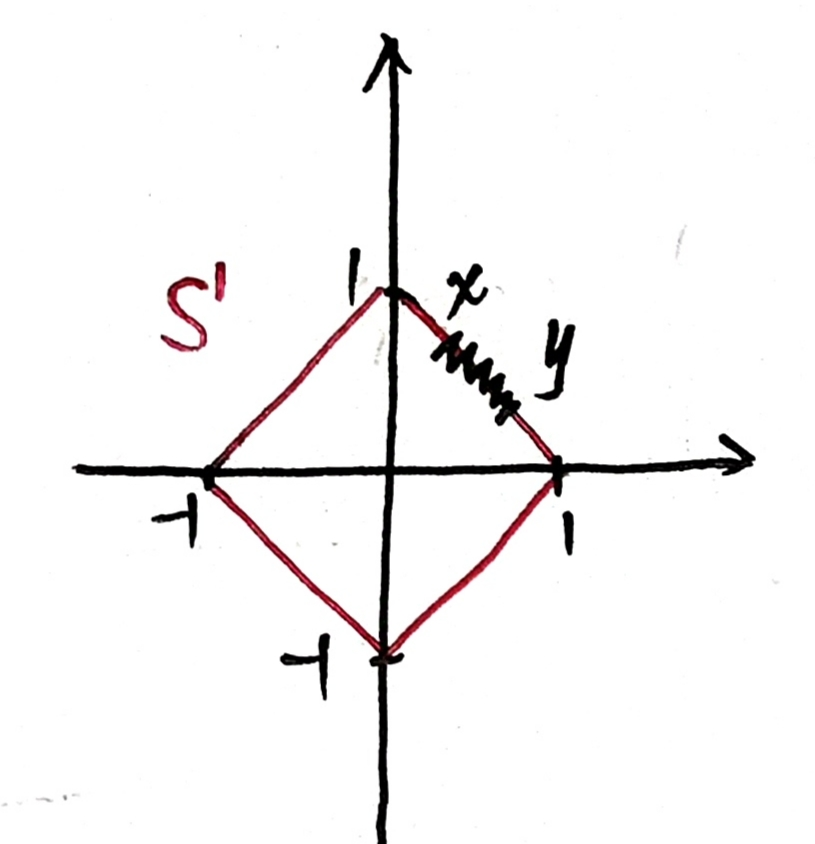
\includegraphics[width=0.3\linewidth]{figure/2.3-1}
					\caption{$(\R^2 , \Vert \cdot \Vert_1)$ 非严格凸}
					\label{pic : 2.3-1} % 添加图像引用标签
				\end{figure}
				
				\begin{center}
					($(\R^2 , \Vert \cdot \Vert_1)$ 中的单位球面$S^1$ 为红线所示正方形)
				\end{center}
			\end{example}
		\end{rmk}
	\end{defn}

	\vspace{2em}
	
	下面给出\textbf{严格凸的等价条件}, 即\textbf{范数三角不等式取等 $\Leftrightarrow$ 两向量同向共线}. 
	
	\newpage
	
	\begin{proposition}\label{prop 2.3.1}
		\textbf{[严格凸的等价条件]}. \\
		Suppose $(X , \Vert \cdot \Vert) \in B^*$, then $X$ 严格凸 $\Leftrightarrow$ For $\forall x , y \neq 0$, 
		\[ \Vert x + y \Vert = \Vert x \Vert + \Vert y \Vert \,\, \Leftrightarrow \,\, \exists \lambda > 0 , \st x = \lambda y \]
		\begin{center}
			即$x$ 与$y$ 同向共线.
		\end{center}
		
		\vspace{1em}
		
		\begin{proof}
			\begin{enumerate}
				\item[$\Leftarrow$]: $\forall x , y \in X$, $x \neq y$, $\Vert x \Vert = \Vert y \Vert = 1$, 下证:$\Vert \alpha x + (1 - \alpha) y \Vert < 1 , \,\, \forall \alpha \in (0 , 1)$:\\
				Since $x \neq y$, $\Vert x \Vert = \Vert y \Vert = 1$, then $x$ and $y$ \textbf{不}同向共线
				\begin{center}
					(Otherwise if $x = \lambda y , \lambda > 0$, then $\Vert x \Vert = \Vert \lambda y \Vert = \Vert y \Vert \,\, \Rightarrow \,\, \lambda = 1$, 与$x \neq y$ 矛盾)
				\end{center}
				Then $\alpha x$ 与$(1 - \alpha) y$ 也不同向共线, $\forall \alpha \in (0 , 1)$. \\
				根据条件的逆否命题, 
				\[ \Vert \alpha x + (1 - \alpha) y \Vert \neq \alpha \, \Vert x \Vert + (1 - \alpha) \, \Vert y \Vert , \,\, \forall \alpha \in (0 , 1) \]
				Thus by the \textbf{triangle inequality (Def \ref{def 2.1.1} (\rmnum{3}))}, 
				\[ \Vert \alpha x + (1 - \alpha) y \Vert < \alpha \, \Vert x \Vert + (1 - \alpha) \, \Vert y \Vert , \,\, \forall \alpha \in (0 , 1) \]
				Therefore, $X$ 严格凸. 
				
				\vspace{4em}
				
				\item[$\Rightarrow$]: Suppose $x , y \neq 0$, $\Vert x + y \Vert = \Vert x \Vert + \Vert y \Vert$, 下证:$x , y$ 同向共线:\\
				Since $\Vert x + y \Vert = \Vert x \Vert + \Vert y \Vert$, then
				\[ 
				\frac{\Vert x + y \Vert}{\Vert x \Vert + \Vert y \Vert} 
				= \left\Vert \frac{x}{\Vert x \Vert + \Vert y \Vert} + \frac{y}{\Vert x \Vert + \Vert y \Vert}  \right\Vert 
				= 1
				\]
				Since
				\[ \frac{x}{\Vert x \Vert + \Vert y \Vert} 
				= \frac{x}{\Vert x \Vert} \cdot \frac{\Vert x \Vert}{\Vert x \Vert + \Vert y \Vert} 
				= \alpha \, \frac{x}{\Vert x \Vert} \]
				where $\alpha = \dfrac{\Vert x \Vert}{\Vert x \Vert + \Vert y \Vert} \in (0 , 1)$. Similarly, we can get
				\[ \frac{y}{\Vert x \Vert + \Vert y \Vert} = (1 - \alpha) \, \frac{y}{\Vert y \Vert} , \,\, \text{where} \,\, \alpha = \frac{\Vert x \Vert}{\Vert x \Vert + \Vert y \Vert} \]
				Thus
				\[ 
				\frac{\Vert x + y \Vert}{\Vert x \Vert + \Vert y \Vert} 
				= \left\Vert \alpha \, \frac{x}{\Vert x \Vert} + (1 - \alpha) \, \frac{y}{\Vert y \Vert} \right\Vert 
				= 1 
				\]
				而又因为 $X$ 严格凸, $\left\Vert \dfrac{x}{\Vert x \Vert} \right\Vert = \left\Vert \dfrac{y}{\Vert y \Vert} \right\Vert = 1$, thus 
				\[ \frac{x}{\Vert x \Vert} = \frac{y}{\Vert y \Vert} \,\, \Rightarrow \,\, x = \frac{\Vert x \Vert}{\Vert y \Vert} y \]
				Therefore, $x , y$ 同向共线.
			\end{enumerate}
		\end{proof}
	\end{proposition}

	\vspace{6em}
	
	下面我们给出有关严格凸的一个命题, 它给出了\textbf{最佳逼近问题}\footnote{可参考\textbf{《泛函分析讲义》 ——张恭庆、林源渠 P39 $\S 4.5$ \underline{应用:最佳逼近问题}}.}的存在唯一性的理论依据. 
	
	\vspace{1em}
	
	\begin{proposition}\label{prop 2.3.2}
		\textbf{[最佳逼近问题解的存在唯一性]}. \\
		Suppose $(X , \Vert \cdot \Vert) \in B^*$. If $X$ 严格凸, $X_0 \subset X$ 为有限维子空间, then for $\forall x \in X$, $\exists$ 唯一的$x_0 \in X_0$, $\st$
		\[ \Vert x - x_0 \Vert = dist(x , X_0) \]
		
		\vspace{4em}
		
		\begin{rmk}
			\begin{itemize}
				\item 作为该命题的一个直接推论, 考虑
				\begin{center}
					\textbf{区间$[a , b]$ 上连续函数的多项式最优逼近问题}
				\end{center}
			即在无穷范数意义下$(C[a , b] , \Vert \cdot \Vert_\infty)$, $\forall f \in C[a , b]$, 对于有限维子空间$P[a , b] = span\{ 1 , x , x^2 , \cdots , x^n \}$, 根据该命题, 依赖$(C[a , b] , \Vert \cdot \Vert_\infty)$ 的\textbf{严格凸性}, 存在唯一的至多$n$次多项式$g_0 \in P[a , b]$, $\st$
			\[ \Vert f - g_0 \Vert_{\infty} = \inf_{g \in P[a , b]} \Vert f - g \Vert_\infty \]
			这样就给出了该最佳逼近问题的\textbf{解的存在唯一性}的理论依据. 
			
			\vspace{6em}
			
			\item 在命题条件中, $X$ 的\textbf{严格凸性}事实上只保证了解的\textbf{唯一性}, 而解的\textbf{存在性}不需要严格凸的保证.
			\end{itemize}
		\end{rmk}
		
		\newpage
		
		\begin{proof}
			\begin{itemize}
				\item \textbf{存在性}:Fix $x \in X$. Since $d = dist(x , X_0) = \underset{y \in X_0}{\inf} {\Vert x - y \Vert}$, then for $\epsilon = \dfrac{1}{n} > 0$, $\exists x_n \in X_0$, $\st$
				\[ d \leq \Vert x - x_n \Vert < d + \frac{1}{n} , \,\, \forall n \in \N \]
				Thus $x_n \in B(x , d + 1) , \,\, \forall n \in \N$. $\{ x_n \}_{n = 1}^{\infty} \subset X_0$ is bounded. \\
				Since $dim(X_0) < \infty$, then By \textbf{有限维赋范空间的等价刻画 (Thm \ref{thm 2.2.6})}, 
				\[ \{ x_n \}_{n = 1}^{\infty} \subset X_0 \,\, \text{bounded} \,\, \Leftrightarrow \,\, \{ x_n \}_{n = 1}^{\infty} \,\, \text{subsequentially compact} \]
				Thus $\exists$ subsequence $\{ x_{n_k} \}_{k = 1}^{\infty} \subset \{ x_n \}_{n = 1}^{\infty}$, $\st x_{n_k} \to x_0 \in X_0$ as $k \to \infty$. \\
				Then $\Vert x - x_0 \Vert = \underset{k \to \infty}{\lim} {\Vert x - x_{n_k} \Vert} = d$.
				
				\vspace{8em}
				
				\item \textbf{唯一性}:反证法. Assume $\exists x_0 , y_0 \in X_0$, $x_0 \neq y_0$, $\st \Vert x - x_0 \Vert = \Vert x - y_0 \Vert = d$. \\
				For $\forall \alpha \in (0 , 1)$, 
				\begin{align}
				\Big\Vert x - [\alpha x_0 + (1 - \alpha) y_0] \Big\Vert 
				&= \Big\Vert \alpha (x - x_0) + (1 - \alpha) (x - y_0) \Big\Vert \\
				&\leq \alpha \Vert x - x_0 \Vert + (1 - \alpha) \Vert x - y_0 \Vert \\
				&= d
				\end{align}
				Since $\alpha x_0 + (1 - \alpha) y_0 \in X_0$, then by the \textbf{minimality of $d$}, 
				\[ \Big\Vert x - [\alpha x_0 + (1 - \alpha) y_0] \Big\Vert = d , \,\, \forall \alpha \in (0 , 1) \]
				i.e.
				\[ \left\Vert \alpha \, \frac{x - x_0}{d} + (1 - \alpha) \, \frac{x - y_0}{d} \right\Vert = 1 , \,\, \forall \alpha \in (0 , 1) \]
				
				\vspace{2em}
				
				Since $X$ 严格凸, $\left\Vert \dfrac{x - x_0}{d} \right\Vert = \left\Vert \dfrac{x - y_0}{d} \right\Vert = 1$, $\dfrac{x - x_0}{d} \neq \dfrac{x - y_0}{d}$, then 
				
				\[ \left\Vert \alpha \, \frac{x - x_0}{d} + (1 - \alpha) \, \frac{x - y_0}{d} \right\Vert < 1 , \,\, \forall \alpha \in (0 , 1) \]
				which contradicts to the upper conclusion. Therefore, $x_0 = y_0$.
			\end{itemize}
		\end{proof}
	\end{proposition}

\newpage

\section{$B^*$ 空间的商空间}
	这一节我们来介绍\textbf{赋范空间的商空间}, 在其上定义运算与范数, 并说明其成为\textbf{完备赋范空间 ($B$ 空间)}. 
	
	\vspace{1em}
	
	\begin{defn}\label{def 2.4.1}
		Suppose $(X , \Vert \cdot \Vert) \in B^*$, $X_0 \subset X$ 为闭子空间, 定义等价关系
		\[ x \sim y \,\, \Leftrightarrow \,\, x - y \in X_0 \]
		记$x + X_0$ 表示$x \in X$ 所在等价类, 从而得到商集$X / X_0$, 即
		\[ X / X_0 \coloneqq \{ x + X_0 \mid x \in X \} \]
		引入$X / X_0$ 中加法和数乘运算如下:
		\[ 
		 \begin{cases}
		 	(x + X_0) + (y + X_0) \coloneqq (x + y) + X_0 , \,\, \forall x , y \in X \\
		 	k \cdot (x + X_0) \coloneqq kx + X_0 , \,\, \forall k \in \mathbb{K} , \,\, \forall x \in X
		 \end{cases}
		 \]
		 不难证明此时$X / X_0$ 满足线性空间的要求. 再引入范数
		 \[ \Vert x + X_0 \Vert_0 \coloneqq dist(x , X_0) = \inf_{y \in X_0} \Vert x - y \Vert , \,\, \forall x \in X \]
		 则$(X / X_0 , \Vert \cdot \Vert_0) \in B^*$, 称$(X / X_0 , \Vert \cdot \Vert_0)$ 为关于$X$ 的\underline{\textcolor{blue}{\textbf{商空间}}}. 
		 
		 \vspace{4em}
		 
		 \begin{rmk}
		 	\begin{itemize}
		 		\item 由于$X_0 \subset X$ 为子空间, 不难验证二元关系$\sim$ 满足:\textbf{自反性、对称性、传递性}. 
		 		
		 		\vspace{4em}
		 		
		 		\item 下面来证明上述定义的$\Vert \cdot \Vert_0$ 满足\textbf{范数的三条公理 (Def \ref{def 2.1.1})}:
		 		
		 		\vspace{4em}
		 		
		 		\begin{proof}
		 			由于$\Vert \cdot \Vert$ 满足正定性, 因此$\Vert \cdot \Vert_0$ 显然满足\textbf{正定性}. \\
		 			For $\forall k \in \mathbb{K}$, $k \neq 0$, 
		 			\begin{align}
		 				\Vert k \cdot (x + X_0) \Vert_0 
		 				= \Vert kx + X_0 \Vert_0 
		 				&= \inf_{y \in X_0} \Vert kx - y \Vert \\
		 				&= \left| k \right| \inf_{\tfrac{y}{k} \in X_0} \Vert x - \frac{y}{k} \Vert \\
		 				&= \left| k \right| \inf_{z \in X_0} \Vert x - z \Vert 
		 				= \left| k \right| \cdot \Vert x + X_0 \Vert_0 , \,\, \forall x \in X
		 			\end{align}
	 				Thus $\Vert \cdot \Vert_0$ 满足\textbf{绝对齐性}. 
	 				\begin{align}
	 					\Vert (x + X_0) + (y + X_0) \Vert_0 
	 					= \Vert (x + y) + X_0 \Vert_0 
	 					&= \inf_{z \in X_0} \Vert (x + y) - z \Vert \\
	 					&= \inf_{\substack{x_0 \in X_0 \\ y_0 \in X_0}} \Vert (x + y) - (x_0 + y_0) \Vert \\
	 					&\leq \inf_{\substack{x_0 \in X_0 \\ y_0 \in X_0}} \left( \Vert x - x_0 \Vert + \Vert y - y_0 \Vert \right) \\
	 					&= \inf_{y_0 \in X_0} \left[ \inf_{x_0 \in X_0} \Big( \Vert x - x_0 \Vert + \Vert y - y_0 \Vert \Big) \right] \\
	 					&= \inf_{y_0 \in X_0} \left( \Vert y - y_0 \Vert + \inf_{x_0 \in X_0} \Vert x - x_0 \Vert \right) \\
	 					&= \inf_{x_0 \in X_0} \Vert x - x_0 \Vert + \inf_{y_0 \in X_0} \Vert y - y_0 \Vert \\
	 					&= \Vert x + X_0 \Vert_0 + \Vert y + X_0 \Vert_0 , \,\, \forall x , y \in X
	 				\end{align}
 					Therefore, $\Vert \cdot \Vert_0$ satisfies the \textbf{triangle inequality}, $(X / X_0 , \Vert \cdot \Vert_0) \in B^*$.
		 		\end{proof}
	 		\end{itemize}
		 \end{rmk}
	\end{defn}

\newpage

\subsection{商空间的完备性}
	在前面我们给出了$B^*$ 空间$(X , \Vert \cdot \Vert)$ 上商空间$(X / X_0 , \Vert \cdot \Vert_0)$ 的定义, 并说明了其为\textbf{赋范空间 ($B^*$ 空间)}. 在这一小节我们将揭示, 如果$X \in B$ 完备, 则\textbf{其上定义的商空间均为完备赋范空间 ($B$ 空间)}. 
	
	\vspace{1em}
	
	\begin{thm}\label{thm 2.4.1}
		\textbf{[商空间的完备性]}. 
		\begin{center}
			\textbf{设$(X , \Vert \cdot \Vert) \in B , \,\, X_0 \subset X$ 为闭子空间, 则$(X / X_0 , \Vert \cdot \Vert_0) \in B$.}
		\end{center}
		
		\vspace{4em}
		
		\begin{proof}
			$\forall$ Cauchy sequence $\{ x_n + X_0 \}_{n = 1}^{\infty} \subset X / X_0$, i.e. $\forall \epsilon > 0$, $\exists N_\epsilon \in \N$, $\st$
			\[ \Big\Vert (x_n + X_0) - (x_m + X_0) \Big\Vert_0 < \epsilon , \,\, \forall m , n \geq N_\epsilon \]
			For $\epsilon = \dfrac{1}{2}$, $\exists n_1 \in \N$, $\st$
			\[ \Big\Vert (x_n + X_0) - (x_m + X_0) \Big\Vert_0 < \frac{1}{2} , \,\, \forall m , n \geq n_1 \]
			For $\epsilon = \dfrac{1}{4}$, $\exists n_2 > n_1$, $\st$
			\[ \Big\Vert (x_n + X_0) - (x_m + X_0) \Big\Vert_0 < \frac{1}{4} , \,\, \forall m , n \geq n_2 \]
			\begin{center}
				$\cdots$
			\end{center}
			Then we get a subsequence $\{ x_{n_k} + X_0 \}_{k = 1}^{\infty} \subset \{ x_n + X_0 \}_{n = 1}^{\infty}$, $\st$
			\[ \Big\Vert (x_{n_{k + 1}} + X_0) - (x_{n_k} + X_0) \Big\Vert_0 < \frac{1}{2^k} , \,\, \forall k \in \N \]
			i.e.
			\[ dist(x_{n_{k + 1}} - x_{n_k} , X_0) = \inf_{y \in X_0} \Vert (x_{n_{k + 1}} - x_{n_k}) - y \Vert < \frac{1}{2^k} \]
			Thus $\exists y_k \in X_0$, $\st$
			\[ \Vert x_{n_{k + 1}} - x_{n_k} - y_k \Vert < \frac{1}{2^k} , \,\, \forall k \in \N \]
			Then the series $\overset{\infty}{\underset{k = 1}{\sum}} \Big( x_{n_{k + 1}} - x_{n_k} - y_k \Big)$ 绝对收敛. \\
			Since $(X , \Vert \cdot \Vert) \in B$ complete, then by \textbf{$B^*$ 空间完备的等价刻画 (Thm \ref{thm 2.1.2})}, 级数收敛, \\
			即$\exists z \in X$, $\st$
			\[
				\sum_{k = 1}^{\infty} \Big( x_{n_{k + 1}} - x_{n_k} - y_k \Big) = z
			\]
			i.e.
			\[
				\sum_{k = 1}^{N - 1} \Big( x_{n_{k + 1}} - x_{n_k} - y_k \Big) = x_{n_N} - x_{n_1} - \sum_{k = 1}^{N - 1} y_k \longrightarrow z \,\, \text{as} \,\, N \to \infty 
			\]
			Thus
			\[ x_{n_N} - \sum_{k = 1}^{N - 1} y_k \to z + x_{n_1} \,\, \text{as} \,\, N \to \infty \]
			Consider 自然同态
			\begin{align}
				\pi : X &\longrightarrow X / X_0 \\
				x &\longmapsto x + X_0
			\end{align}
			Since $X_0 \subset X$ 为子空间, then $0 \in X_0$. Thus for $\forall \epsilon > 0$, $\exists \delta = \epsilon > 0$, $\st$
			\begin{align}
				\Vert \pi(x) - \pi(y) \Vert_0 
				= \Vert (x - y) + X_0 \Vert_0 
				&= dist(x - y , X_0) \\
				&= \inf_{z \in X_0} \Vert (x - y) - z \Vert \\
				&\leq \Vert x - y \Vert + \inf_{z \in X_0} \Vert z \Vert \\
				&= \Vert x - y \Vert 
				< \epsilon , \,\, \forall \Vert x - y \Vert < \delta
			\end{align}
			Thus $\pi$ is continuous. Since
			\[ x_{n_N} - \sum_{k = 1}^{N - 1} y_k \to z + x_{n_1} \,\, \text{as} \,\, N \to \infty \]
			Then
			\[ \pi \left( x_{n_N} - \sum_{k = 1}^{N - 1} y_k \right) \to \pi(z + x_{n_1}) \]
			i.e.
			\[ \left( x_{n_N} - \sum_{k = 1}^{N - 1} y_k \right) + X_0 \to (z + x_{n_1}) + X_0 \]
			Since $y_k \in X_0 , \,\, \forall k \in \N$, then
			\[ \left( x_{n_N} - \sum_{k = 1}^{N - 1} y_k \right) + X_0 = x_{n_N} + X_0 \to (z + x_{n_1}) + X_0 \,\, \text{as} \,\, N \to \infty \]
			Therefore, $\{ x_{n_k} + X_0 \}_{k = 1}^{\infty}$ converges to $(z + x_{n_1}) + X_0 \in X / X_0$ \\
			$\Rightarrow \,\,$ Cauchy sequence $\{ x_n + X_0 \}_{n = 1}^{\infty}$ converges \\
			$\Rightarrow \,\, (X / X_0 , \Vert \cdot \Vert_0)$ complete
		\end{proof}
	\end{thm}






	%  ############################
	\ifx\allfiles\undefined
\end{document}
\fi